% !Tex root = vaje.tex
\chapter{Polinomi}
\label{cha:polinomi}

\section{Pregled snovi}
\label{sec:polinomi-pregled-snovi}

Foo.

\section{Vaje}
\label{sec:polinomi-funkcije-vaje}

%%%%%%%%%%%%%%%%%%%%%%%%%%%%%%%%%%%%%%%%%%%%%%%%%%%%%%%%%%%%%%%%%%%%%%
% Odpremo datoteko, v katero se bodo zapisali odgovori za
% to poglavje.

% Določimo ime datoteke, v katero se bodo pisali odgovori.
% Vsako poglavje mora imeti svojo datoteko.
\def\datotekaOdgovori{odgovori-polinomi}

% Odpremo datoteko z odgovori.
\Opensolutionfile{odgovor}[\datotekaOdgovori]


\begin{vaja}
Zgled risanja polinomov:
Narišite graf polinoma $p(x)=x^3-3x+2$.
Potrebujemo:
\begin{itemize}
\item začetno vrednost
\item ničle polinoma
\item kako se funkcija obnaša v neskončnosti
\item ekstreme funkcije
\end{itemize}

Začetna vrednost je enaka $p(0)=2$
Da dobimo ničle, polinom najprej razstavimo s pomočjo Hornerjevega algoritma in dobimo 3 ničle:
$x_{1,2}=1$ (soda) in $x_3=-2$ (liha). Pri sodi ničli se funkcija samo dotakne $x-osi$ in je ne seka, pri lihi pa
funkcija seka $x-os$.
Nato še pogledamo, kako se funkcija obnaša na robovih definicijskega območja. Vidimo, da pri $+\infty$ se graf bliža $+\infty$,
pri $-\infty$ pa $-\infty$.
Zanimajo nas še lokalni ekstremi funkcije, zato izračunamo odvod funkcije: $p\prime(x)=3x^2-3$. Zanima nas, kdaj je enak $0$. Dobimo enačbo $3x^2-3=0$ in dobimo rešitvi $x_1=1$ in $x_2=-1$. Izračunamo še vrednost funkcije v teh točkah in narišemo graf $p(x)$.


\definecolor{qqwuqq}{rgb}{0,0.39215686274509803,0}
\definecolor{cqcqcq}{rgb}{0.7529411764705882,0.7529411764705882,0.7529411764705882}

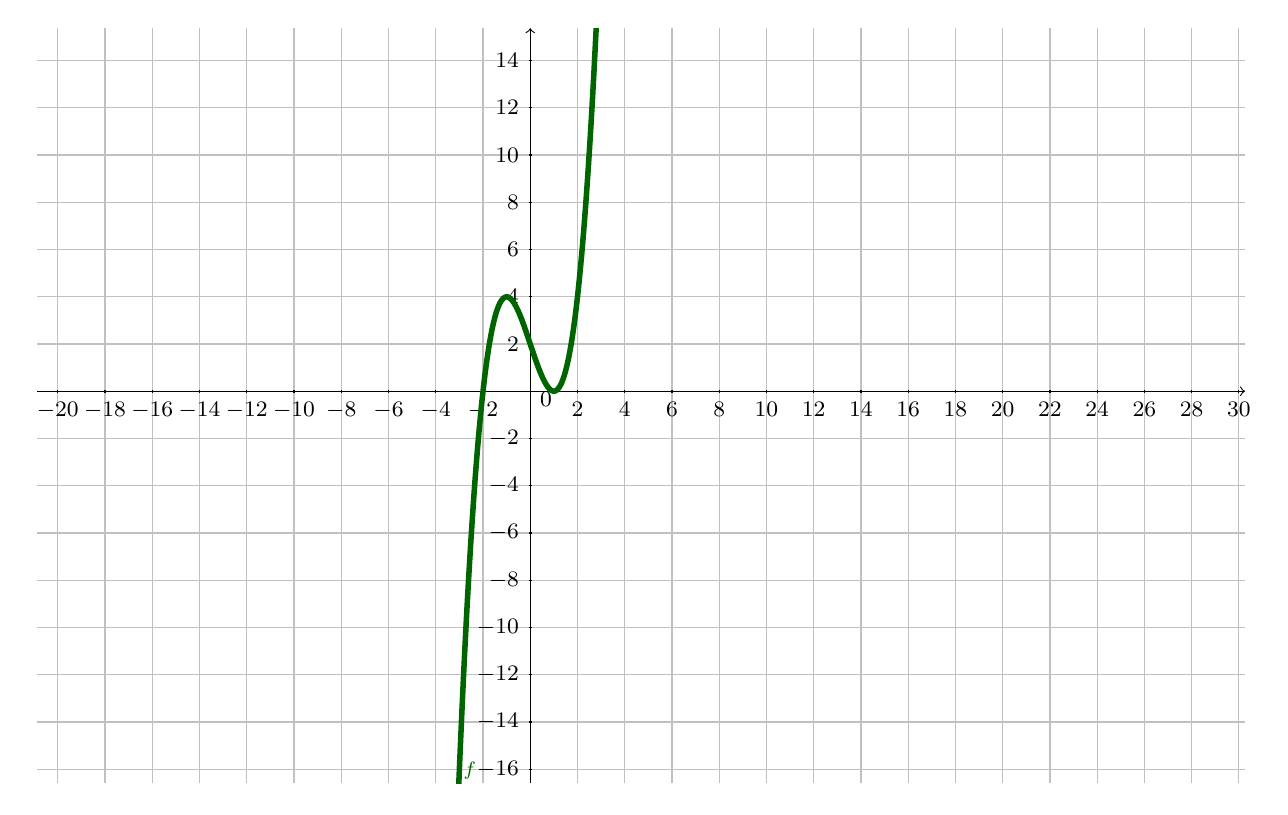
\begin{tikzpicture}[scale=0.3][line cap=round,line join=round,>=triangle 45,x=1cm,y=1cm]

\draw [color=cqcqcq,, xstep=2cm,ystep=2cm] (-20.867622516121354,-16.60212053777514) grid (30.25787851421771,15.368179578822133);

\draw[->,color=black] (-20.867622516121354,0) -- (30.25787851421771,0);
\foreach \x in {-20,-18,-16,-14,-12,-10,-8,-6,-4,-2,2,4,6,8,10,12,14,16,18,20,22,24,26,28,30}
\draw[shift={(\x,0)},color=black] (0pt,2pt) -- (0pt,-2pt) node[below] {\footnotesize $\x$};
\draw[->,color=black] (0,-16.60212053777514) -- (0,15.368179578822133);
\foreach \y in {-16,-14,-12,-10,-8,-6,-4,-2,2,4,6,8,10,12,14}
\draw[shift={(0,\y)},color=black] (2pt,0pt) -- (-2pt,0pt) node[left] {\footnotesize $\y$};
\draw[color=black] (0pt,-10pt) node[right] {\footnotesize $0$};\clip(-20.867622516121354,-16.60212053777514) rectangle (30.25787851421771,15.368179578822133);
\draw[line width=2pt,color=qqwuqq,smooth,samples=100,domain=-7.867622516121354:7.25787851421771] plot(\x,{(\x)^(3)-3*(\x)+2});

\begin{scriptsize}
\draw[color=qqwuqq] (-2.5555202341463437,-16.045675440809045) node {$f$};
\end{scriptsize}

\end{tikzpicture}


\end{vaja}

\begin{vaja}
1. naloga iz risanja polinomov:
Narišite graf polinoma $p(x)=-6x^3+21x^2-21x+6$. Pokažite, da v točki z absciso $\frac{3}{2}$ graf polinoma 
seka simetralo lihih kvadrantov. Zapišite še preostali presečišči grafa polinoma s simetralo lihih kvadrantov.



  \begin{odgovor}
1. naloga: %128.naloga

  \end{odgovor}

\end{vaja}



\begin{vaja}

Zgled bisekcije:
Poiščimo iracionalno ničlo $x_0$ polinoma $p(x)=x^5+2x-1$ na desetinko natančno.

Najprej izberemo začetni interval $[a,b]$, da je $p(a)p(b)<0$. Ker je $p(0)=-1<0$ in $p(1)=2>0$, 
vemo, da je ničla nekje na intervalu $[0,1] \Rightarrow$ \\
ničla bo $0,...$ Razpolovna točka tega intervala je $0,5$. \\
$p(0,5)\doteq 0,03>0$, torej je ničla na intervalu $[0;0,5] \Rightarrow$ \\

ničla bi $0,0...$ ali $0,1...$ ali $0,2...$ ali $0,3...$ ali $0,4...$ Razpolovna točka tega intervala je $0,25$.

$p(0,25)\doteq-0,5<0$, torej je ničla na intervalu $[0,25;0,5] \Rightarrow$ \\
ničla bo $0,2...$ ali $0,3...$ ali $0,4...$ Razpolovna točka tega intervala je $0,375$.

$p(0,375)\doteq -0,24<0$, torej je ničla na intervalu $[0,375;0,5] \Rightarrow$ \\
ničla bo $0,3...$ ali $0,4...$ Razpolovna točka tega intervala je $0,4375$.

$p(0,4375)\doteq -0,11<0$, torej je ničla na intervalu $[0,4375;0,5] \Rightarrow$ \\
ničla bo $0,4...$ (prvo decimalno mesto je znano). Razpolovna točka je $0,46875$.

$p(0,46875)\doteq -0,04<0$, torej je ničla na intervalu $[0,46875;0,5] \Rightarrow$ \\
ničla bo $0,46...$ ali $0,47...$ ali $0,48...$ ali $0,49$...

Bisekcijo bi lahko še nadaljevali in bi dobili še naslednja decimalna mesta.
Iracionalna ničla danega polinoma je med $0,47$ in $0,50$.



\end{vaja}

\begin{vaja}
Dan je polinom $p(x)=4x^3-2x^2-x+6$. Z bisekcijo na štiri mesta natančno poiščite ničlo
polinoma $p$ na intervalu $[-2,-1]$.


\begin{odgovor}
Približna vrednost znaša $x\doteq -1,063$.
\end{odgovor}

\end{vaja}




%%%%%%%%%%%%%%%%%%%%%%%%%%%%%%%%%%%%%%%%%%%%%%%%%%%%%%%%%%%%%%%%%%%%%%
% Treba je zapredi datoteko z odgovori

\Closesolutionfile{odgovor}



%%%%%%%%%%%%%%%%%%%%%%%%%%%%%%%%%%%%%%%%%%%%%%%%%%%%%%%%%%%%%%%%%%%%%%
% Odgovori

\section{Odgovori}
\label{sec:polinomi-odgovori}

% Vključimo odgovore.
\input{\datotekaOdgovori}



%%% Local Variables:
%%% mode: latex
%%% TeX-master: "vaje"
%%% End:
